In the paper~\cite{cruz-ppdp14}, the LM virtual machine was measured and
compared against implementations of similar programs but written in other
languages. For instance, the LBP program was found to be around 2 times slower
than GraphLab, while N Queens program was found to be around 10 to 15 slower
than a sequential C implementation. Some of those programs were compared against
a Python implementations and LM faired fairly well. In this section, we measure
the impact of the coordination mechanisms we have implemented for the new
virtual machine.

Fig.~\ref{results:comparison1} shows the comparison between the original virtual
machine and the new virtual machine with coordination mechanisms. All the
programs benchmarked do not use any kind of coordination. As expected, there
is no degration of performance by adding coordination mechanisms.

\begin{figure}[h!]
   \begin{center}
      \subfloat[]{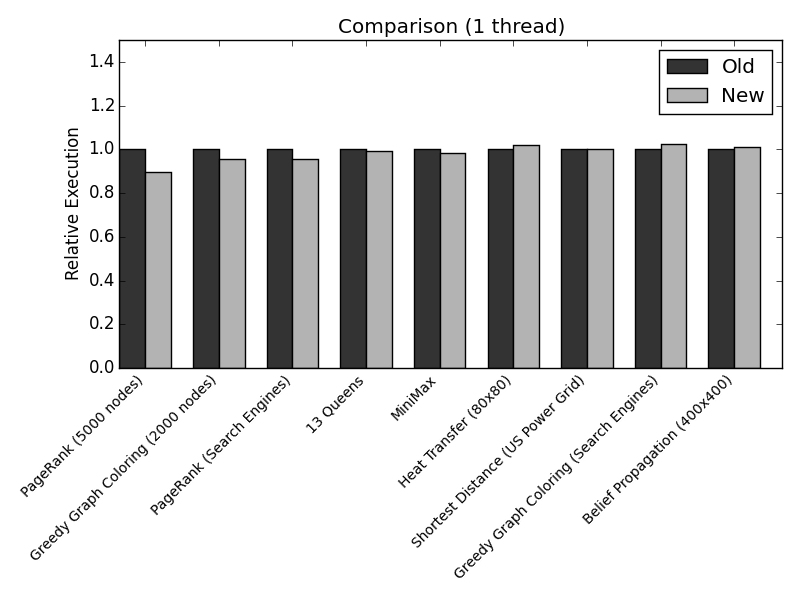
\includegraphics[width=9cm]{results/comparison1.png}}
   \end{center}
   \caption{Measuring the overhead of coordination mechanisms. The \textbf{Old}
   bars represent the performance of the original virtual machine, while
   \textbf{New} is the relative performance of the new version that includes
   coordination mechanisms.}
   \label{results:comparison1}
\end{figure}
